
\chapter{Experimental Evaluation}
\label{ch:eval}

\section{Data Exploration}
\subsection{Adult Dataset}
\label{sec:adult}

\begin{itemize}
    \item Age: The age of the individual (Positive integer)
    \item Work class: The sector the individual works in (8 Categories)
    \item fnlgwgt: A weight determined by the census bureau (Positive integer)
    \item Education: Highest educational degree (16 categories)
    \item Educaitional-num: Enumerated education (16 categories)
    \item Marital Status: Marital status of individual (7 Categories)
    \item Occupation: General type of occupation (15 categories)
    \item Relationship: What kind of relationship the individual is to others (6 categories)
    \item Race: What race the individual belongs to (6 Categories)
    \item Gender: Biological sex of the individual (2 Categories)
    \item Capital gain: Capital gain of individual (Positive integer)
    \item Capital loss: Capital loss of the individual (Positive integer)
    \item Native country: Native country of the individual (42 categories)
    \item Income: Whether individual makes more than 50K or not (2 Categories)
\end{itemize}

This dataset consists of mostly categorical attributes which are not ordinal. This makes analysis quite challenging. Many models assume Gaussian distributions, which is not present in the dataset. In this dataset, there are also some sensitive attributes, most notably \emph{Gender} and \emph{Race}. One could also argue that \emph{Marital Status} and \emph{Relationship} could also be sensitive attributes.

In a fair machine learning system, we would expect that the outcome in terms of income does not depend on the race, gender, marital status or relationship or the very least that the decision by the model is independent of the sensitive attributes.

\subsection{Attributes correlated with income}

\begin{table}
    \centering
    \begin{tabular}{lr}
        \toprule
        Attribute &  Correlation \\
        \midrule
        marital-status.Never-married &    -0.318782 \\
        relationship.Own-child       &    -0.225691 \\
        relationship.Not-in-family   &    -0.190372 \\
        occupation.Other-service     &    -0.155254 \\
        relationship.Unmarried       &    -0.143642 \\
        education.HS-grad            &    -0.130706 \\
        race.Black                   &    -0.090448 \\
        education.11th               &    -0.086728 \\
        occupation.Adm-clerical      &    -0.086475 \\
        relationship.Other-relative  &    -0.085601 \\
        \bottomrule
    \end{tabular}
    \caption{Features that are negatively correlated with income.}
    \label{fig:negative_income_correaltion}
\end{table}

\begin{table}
    \centering
    \begin{tabular}{lr}
        \toprule
        Attribute &  Correlation \\
        \midrule
        education.Masters                 &     0.174184 \\
        education.Bachelors               &     0.180371 \\
        occupation.Prof-specialty         &     0.188793 \\
        occupation.Exec-managerial        &     0.210938 \\
        gender.Male                       &     0.214628 \\
        capital-gain                      &     0.223013 \\
        hours-per-week                    &     0.227687 \\
        age                               &     0.230369 \\
        marital-status.Married-civ-spouse &     0.445853 \\
        \bottomrule
    \end{tabular}
    \caption{Features that are positively correlated with income.}
    \label{fig:positive_income_correaltion}
\end{table}

We see  in that there are some categories in the following attributes that are correlated with income

\begin{itemize}
    \item Marital Status
    \item Age
    \item Hours per week
    \item Capital Gain
    \item Occupation
    \item Relationship
    \item Education
    \item Gender
    \item Race
\end{itemize}

We observe that our identified sensitive attributes are correlated with income. The challenge now is that we have to learn a model that does not treat individuals belonging to different classes in the sensitive attribute unfairly.

\section{Experiment 1: FairBN, FairTreeClassifier vs NB}
\label{sec:result:experiment1}

Below we will go through the different results of the first round of experiments. To see the detailed results, these are available in the appendix. See~\ref{app:experiment1}

\begin{figure}
    \centering
    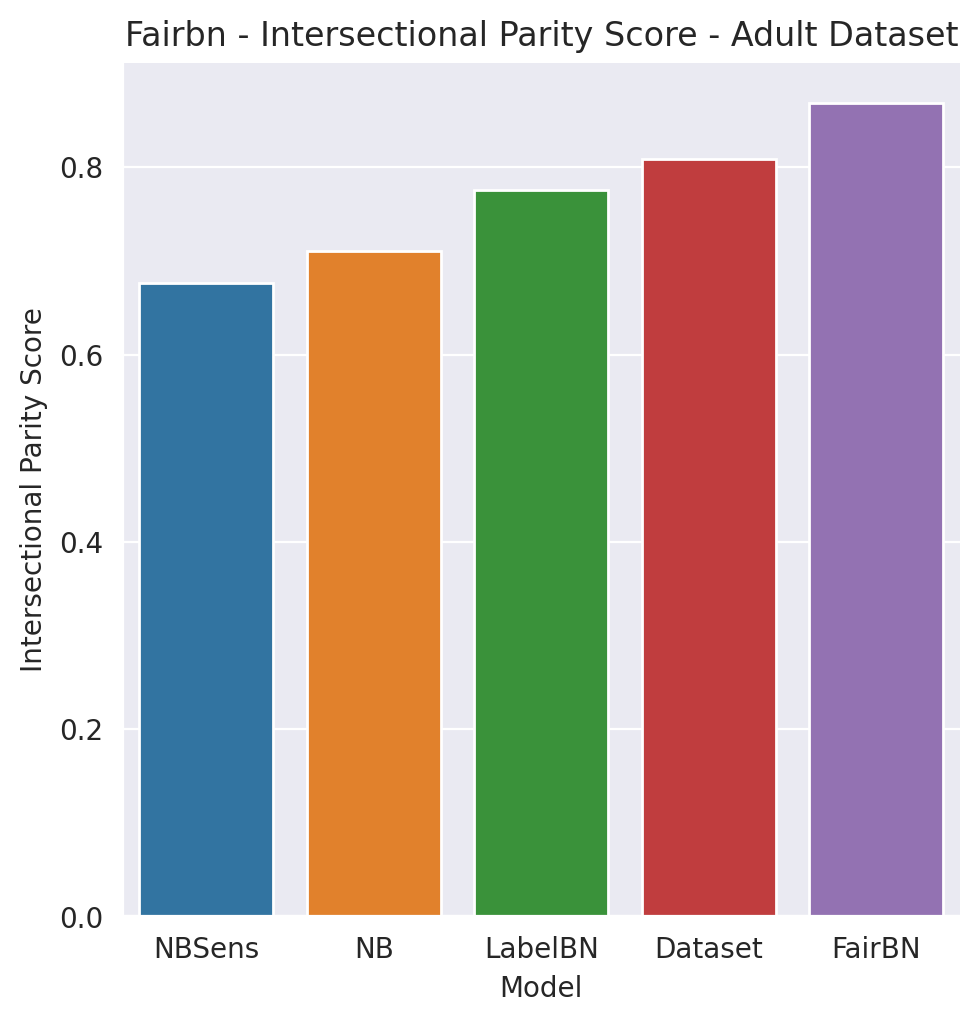
\includegraphics[width=0.49\linewidth]{figures/adult_fairbn_parity.png}
    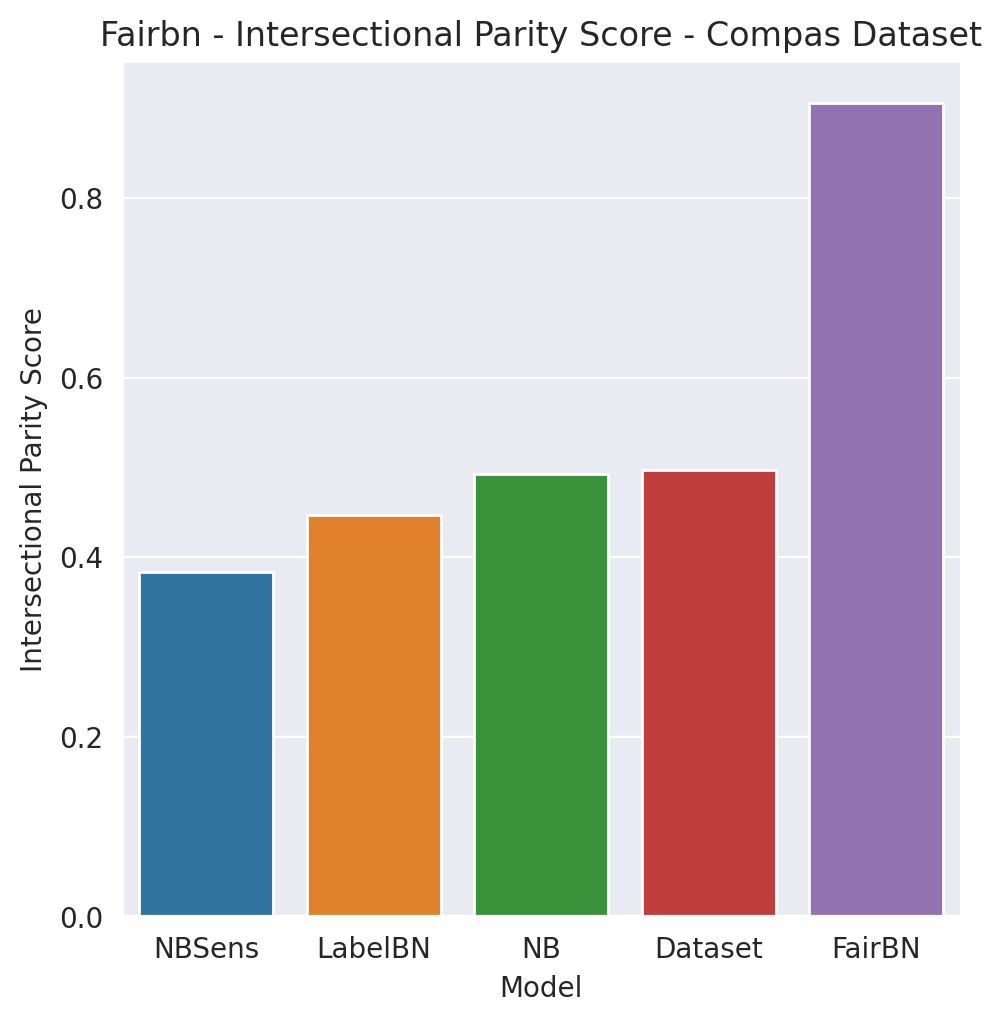
\includegraphics[width=0.49\linewidth]{figures/compas_fairbn_parity.png}
    \caption{Intersectional Parity Score for fair Bayesian network vs naïve bays.}
    \label{fig:exp1fairBNparity}
\end{figure}

\subsection{Fair Bayesian Network}

After training the fair Bayesian network classifier on the adult and Compas dataset, we get an intersectional parity score of $0.87$ and $0.91$ respectively. This is better than the inherent parity score in the dataset labels, which is $0.81$ and $0.51$ respectively. These results and how the different methods compare to one another is shown in figure~\ref{fig:exp1fairBNparity}.

In terms of accuracy and traditional performance of the model, we observe that there is a tradeoff between performance and fairness. This is best shown in the ROC curve shown in figure~\ref{fig:exp1fairBNROC}. There is a slight drop in the fair Bayesian network compared to the naïve Bayes method.

We also observe a quite significant performance difference between the adult dataset and the Compas dataset. Why this is is not explored further in this thesis, as we are interested in seeing differences in performance with respect to fairness.  
\begin{figure}
    \centering
    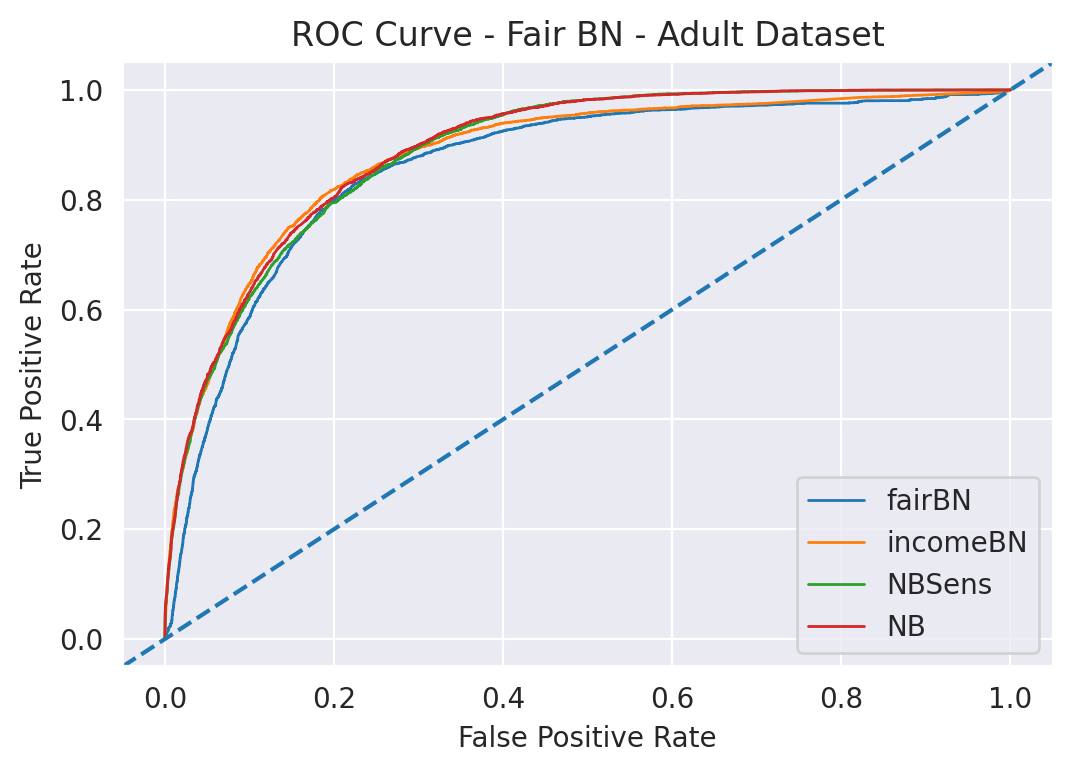
\includegraphics[width=0.49\linewidth]{figures/adult_fairbn_roc.png}
    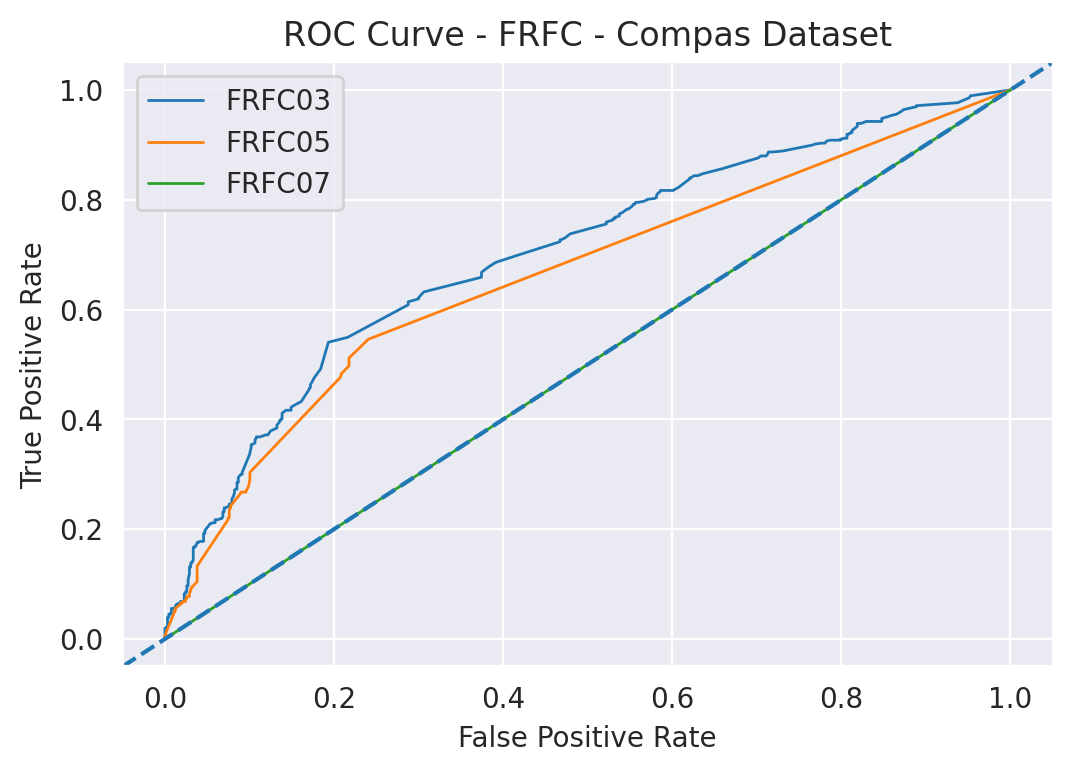
\includegraphics[width=0.49\linewidth]{figures/compas_frfc_roc.png}
    \caption{ROC curve for fair Bayesian network vs naïve Bayes.}
    \label{fig:exp1fairBNROC}
\end{figure}

\subsection{Fair Random Forest Classifier}

We ran the same experiments using their classifier on the adult dataset and Compas dataset. Rather interestingly, we do not observe any improvement in intersectional parity in the adult dataset for any of the methods, with the inherent intersectional parity for the dataset being $0.810$ and the best fair random forest classifier with $\Theta = 0.3$ having an intersectional parity of $0.78$, which is counterintuitive to the claimed meaning behind the hyperparameter $\Theta$ stated by the authors.

\begin{figure}
    \centering
    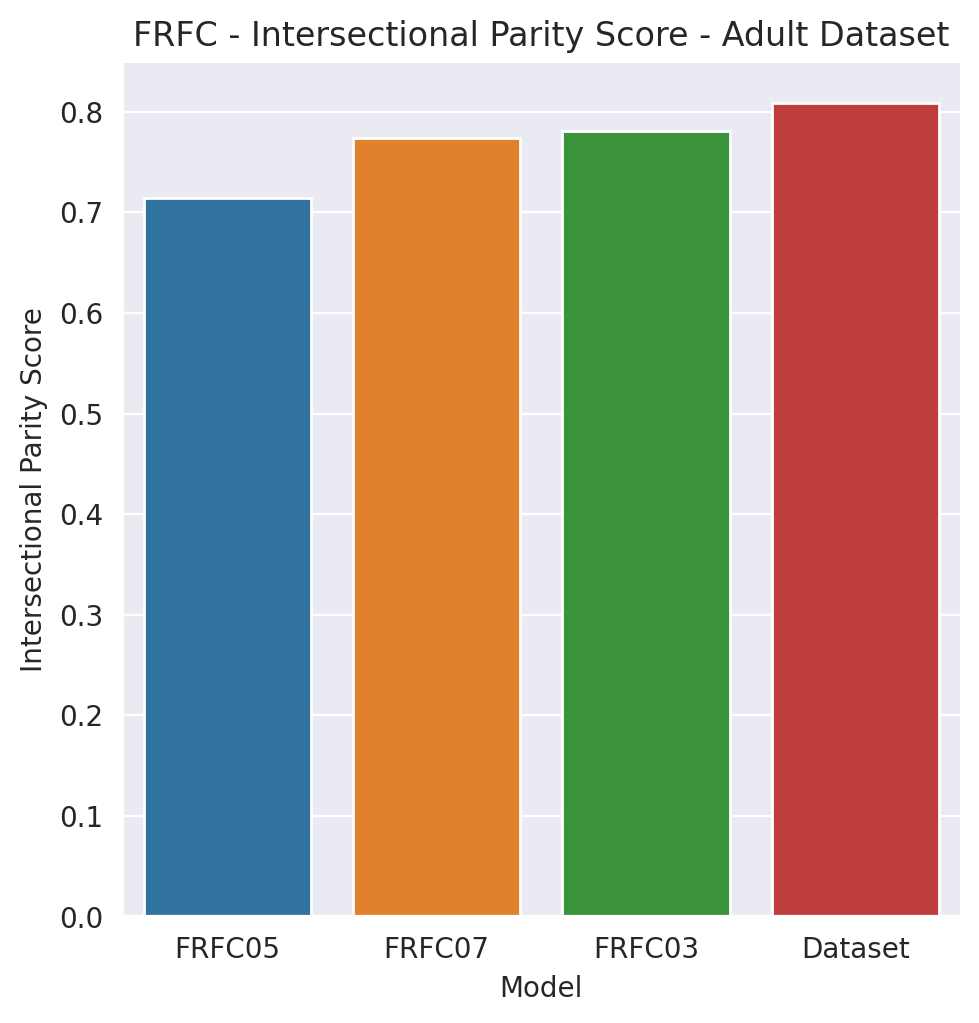
\includegraphics[width=0.49\linewidth]{figures/adult_frfc_parity.png}
    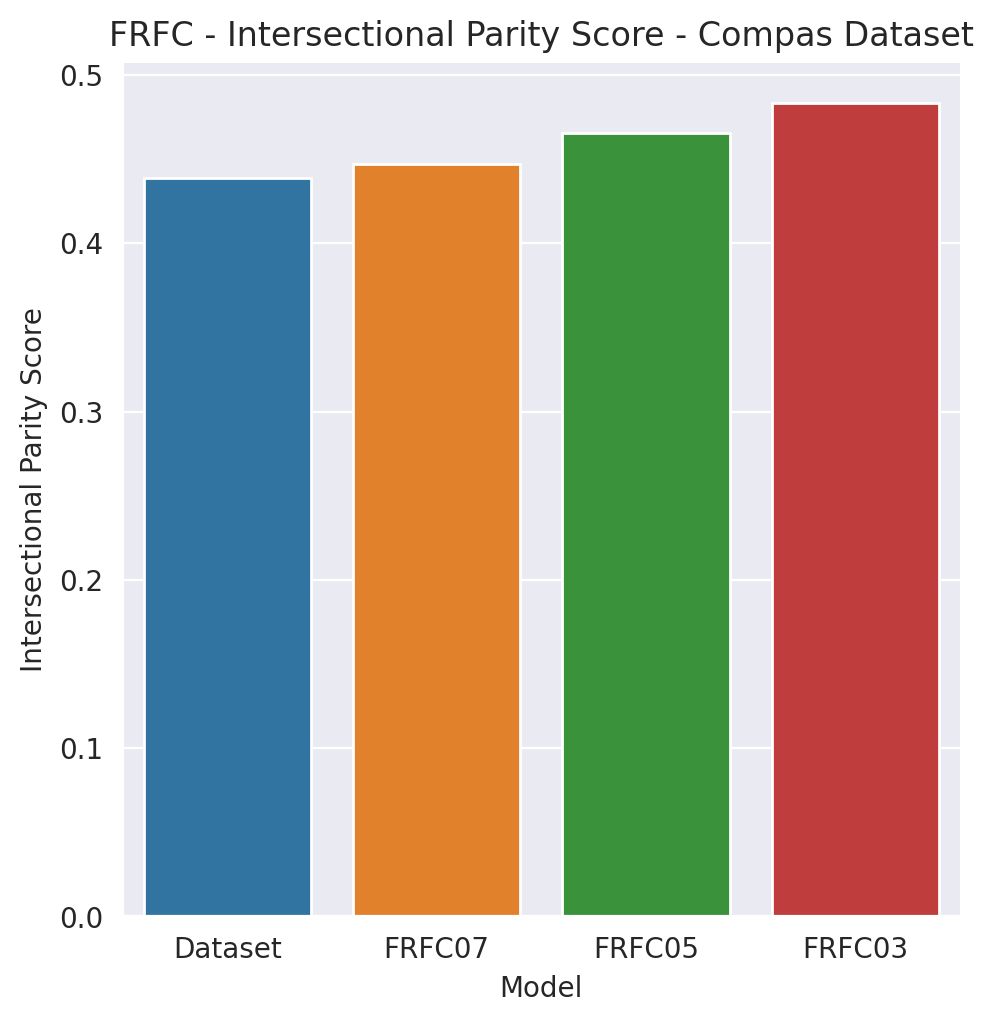
\includegraphics[width=0.49\linewidth]{figures/compas_frfc_parity.png}
    \caption{Parity score for fair random forest classifier.}
    \label{fig:exp1FRFCparity}
\end{figure}

For the Compas dataset, things are looking better with the models with $\Theta \in \{0.3, 0.7\}$ having higher intersectional parity scores than is inherent in the dataset labels. Still, the results given the stated meaning behind $\Theta$ is counterintuitive. The parity scores are shown in figure~\ref{fig:exp1FRFCparity}. The ROC curve for the different datasets is shown in figure~\ref{fig:exp1FRFCROC}

\begin{figure}
    \centering
    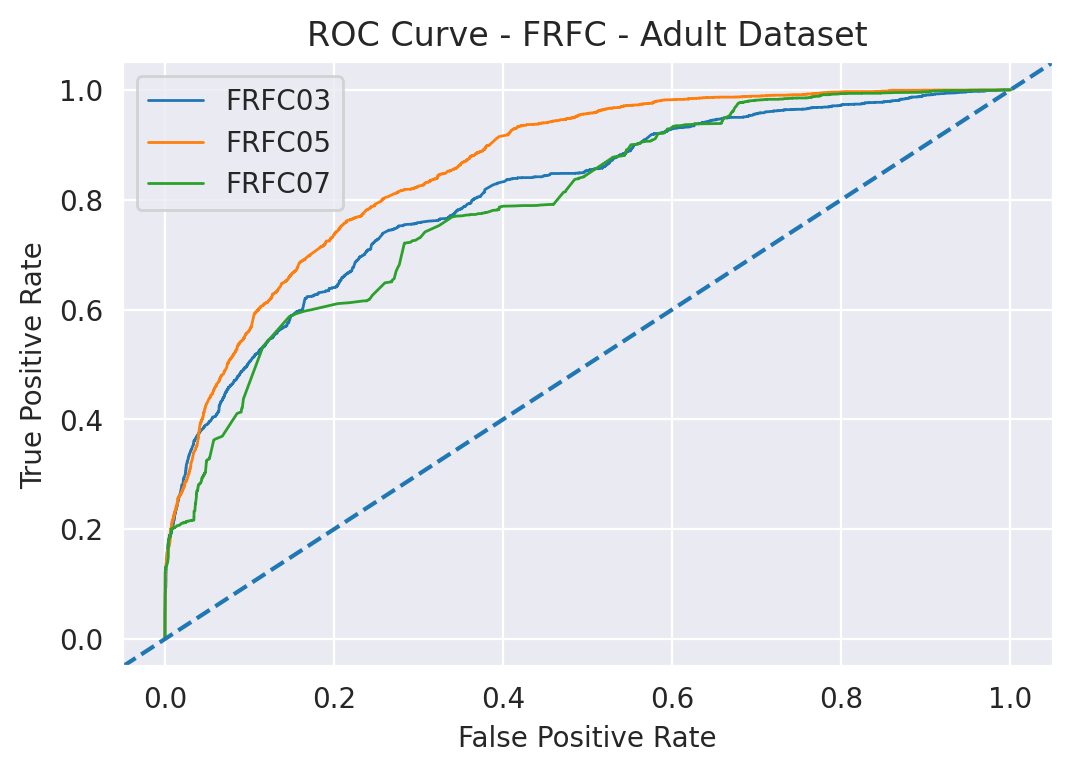
\includegraphics[width=0.49\linewidth]{figures/adult_frfc_roc.png}
    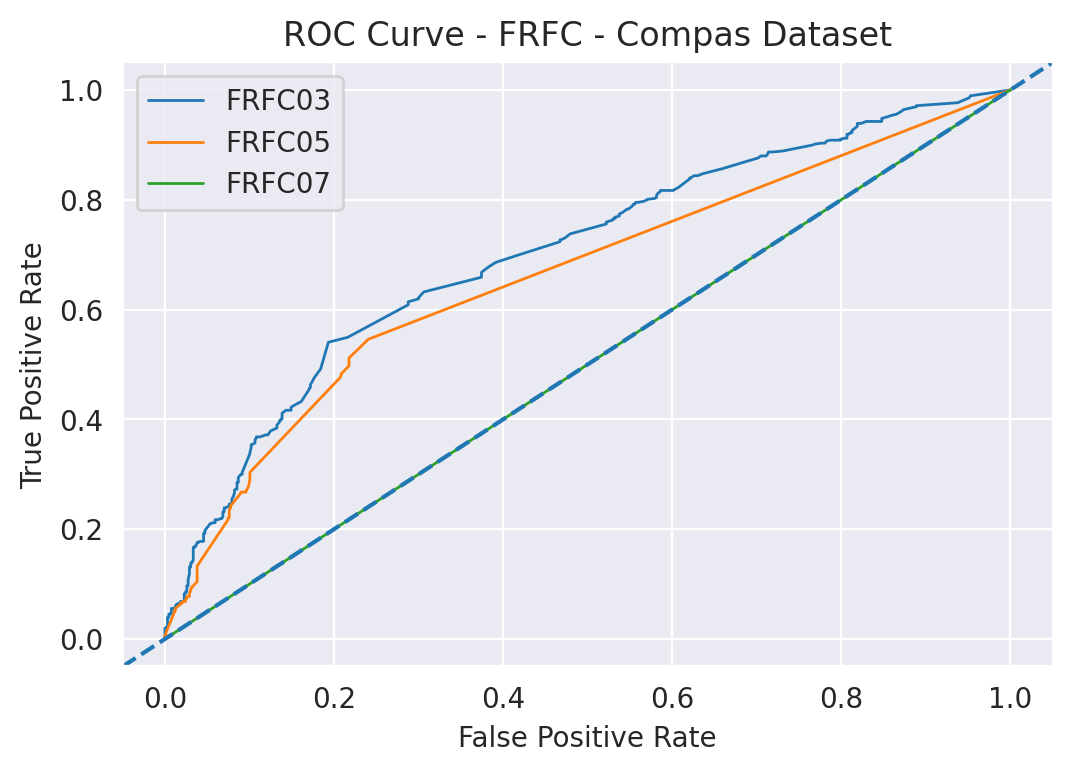
\includegraphics[width=0.49\linewidth]{figures/compas_frfc_roc.png}
    \caption{ROC curve for fair random forest classifier.}
    \label{fig:exp1FRFCROC}
\end{figure}

\section{Counterfactuals}

\subsection{naïve Bayes With Sensitive Attributes}

For the following datapoint:

\resizebox{\textwidth}{!}{
\begin{tabular}{lllllllllll}
\toprule
{} &           age & workclass &  education & marital-status &    occupation & relationship &   race &  gender &          capital-gain & hours-per-week \\
\midrule
46343 &  (31.6, 46.2] &   Private &  Assoc-voc &       Divorced &  Tech-support &    Unmarried &  Black &  Female &  (-4460.355, 16515.0] &   (20.6, 40.2] \\
\bottomrule
\end{tabular}
}

Got the following counterfactuals:

\resizebox{\textwidth}{!}{
\begin{tabular}{lllllllllllrrrr}
\toprule
{} &           age &  workclass &  education &     marital-status &    occupation &   relationship &                race &  gender &        capital-gain & hours-per-week &        O1 &   O2 &  O3 &   O4 \\
\midrule
155 &  (31.6, 46.2] &    Private &  Assoc-voc &  Married-AF-spouse &  Tech-support &      Unmarried &               Black &    Male &  (79128.0, 99999.0] &   (20.6, 40.2] &  0.000000 &  0.7 &   3 &  0.0 \\
162 &  (31.6, 46.2] &    Private &  Assoc-voc &           Divorced &  Adm-clerical &      Unmarried &               Black &    Male &  (79128.0, 99999.0] &   (20.6, 40.2] &  0.000000 &  0.7 &   3 &  0.0 \\
100 &  (31.6, 46.2] &    Private &  Assoc-voc &  Married-AF-spouse &  Adm-clerical &      Unmarried &               Black &    Male &  (58257.0, 79128.0] &   (20.6, 40.2] &  0.000000 &  0.6 &   4 &  0.0 \\
167 &  (31.6, 46.2] &    Private &  Assoc-voc &  Married-AF-spouse &  Adm-clerical &      Unmarried &               Black &    Male &  (79128.0, 99999.0] &   (20.6, 40.2] &  0.000000 &  0.6 &   4 &  0.0 \\
176 &  (31.6, 46.2] &    Private &  Assoc-voc &  Married-AF-spouse &  Adm-clerical &      Unmarried &               Black &    Male &  (58257.0, 79128.0] &   (20.6, 40.2] &  0.000000 &  0.6 &   4 &  0.0 \\
2   &  (60.8, 75.4] &  Local-gov &  Doctorate &           Divorced &             ? &  Not-in-family &  Amer-Indian-Eskimo &  Female &  (79128.0, 99999.0] &   (59.8, 79.4] &  0.000000 &  0.2 &   8 &  0.0 \\
177 &  (31.6, 46.2] &    Private &  Assoc-voc &  Married-AF-spouse &  Tech-support &      Unmarried &               Black &  Female &  (16515.0, 37386.0] &   (20.6, 40.2] &  0.419303 &  0.8 &   2 &  0.0 \\
\bottomrule
\end{tabular}
}


\instructions{
Page budget for Evaluation: 10-15 pages
%
\begin{itemize}
    \item Detail your evaluation methodology, present your results, and provide an analysis of them. Results can be quantitative and/or qualitative (from benchmark, user study, user satisfaction survey, etc.).
    \item It is strongly desired that you have empirical results, nevertheless, this may not be applicable to all types of theses.
\end{itemize}
}

\subsection{naïve Bayes Without Sensitive Attributes}

For the following datapoint:

\resizebox{\textwidth}{!}{
\begin{tabular}{lllllllllll}
\toprule
{} &             age & workclass & education & marital-status & occupation & relationship &   race &  gender &          capital-gain & hours-per-week \\
\midrule
23356 &  (16.927, 31.6] &         ? &   HS-grad &      Separated &          ? &    Unmarried &  Black &  Female &  (-4460.355, 16515.0] &   (20.6, 40.2] \\
\bottomrule
\end{tabular}
} 

We get the following counterfactuals:

\resizebox{\textwidth}{!}{
\begin{tabular}{lllllllllllrrrr}
\toprule
{} &             age &  workclass &  education &     marital-status & occupation &   relationship &                race &  gender &          capital-gain & hours-per-week &        O1 &   O2 &  O3 &   O4 \\
\midrule
128 &  (16.927, 31.6] &  State-gov &    HS-grad &          Separated &          ? &      Unmarried &               Black &    Male &    (79128.0, 99999.0] &   (20.6, 40.2] &  0.000000 &  0.7 &   3 &  0.0 \\
97  &    (31.6, 46.2] &          ? &    HS-grad &          Separated &          ? &  Not-in-family &               Black &    Male &    (79128.0, 99999.0] &   (20.6, 40.2] &  0.000000 &  0.6 &   4 &  0.0 \\
147 &  (16.927, 31.6] &  State-gov &  Doctorate &          Separated &          ? &      Unmarried &               Black &    Male &    (79128.0, 99999.0] &   (20.6, 40.2] &  0.000000 &  0.6 &   4 &  0.0 \\
136 &    (31.6, 46.2] &  State-gov &  Doctorate &  Married-AF-spouse &          ? &        Husband &  Amer-Indian-Eskimo &  Female &  (-4460.355, 16515.0] &   (20.6, 40.2] &  0.165877 &  0.4 &   6 &  0.1 \\
\bottomrule
\end{tabular}
}

\subsection{Fair Bayesian Network}

For the following counterfactual

\resizebox{\textwidth}{!}{
\begin{tabular}{lllllllllll}
\toprule
{} &             age & workclass & education & marital-status & occupation & relationship &   race &  gender &          capital-gain & hours-per-week \\
\midrule
23356 &  (16.927, 31.6] &         ? &   HS-grad &      Separated &          ? &    Unmarried &  Black &  Female &  (-4460.355, 16515.0] &   (20.6, 40.2] \\
\bottomrule
\end{tabular}
}

We get the following counterfactuals

\resizebox{\textwidth}{!}{
\begin{tabular}{lllllllllllrrrr}
\toprule
{} &             age &         workclass &   education & marital-status &       occupation &   relationship &                race &  gender &        capital-gain & hours-per-week &            O1 &   O2 &  O3 &   O4 \\
\midrule
111 &  (16.927, 31.6] &                 ? &        11th &      Separated &                ? &      Unmarried &               Black &  Female &  (79128.0, 99999.0] &   (79.4, 99.0] &  0.000000e+00 &  0.7 &   3 &  0.0 \\
114 &  (16.927, 31.6] &                 ? &     HS-grad &      Separated &                ? &      Unmarried &               White &  Female &  (79128.0, 99999.0] &   (79.4, 99.0] &  0.000000e+00 &  0.7 &   3 &  0.0 \\
162 &  (16.927, 31.6] &                 ? &        11th &      Separated &                ? &      Unmarried &               White &  Female &  (79128.0, 99999.0] &   (20.6, 40.2] &  0.000000e+00 &  0.7 &   3 &  0.1 \\
58  &  (16.927, 31.6] &      Never-worked &     HS-grad &      Separated &                ? &      Unmarried &  Asian-Pac-Islander &  Female &  (58257.0, 79128.0] &   (79.4, 99.0] &  0.000000e+00 &  0.6 &   4 &  0.0 \\
118 &  (16.927, 31.6] &                 ? &  Assoc-acdm &      Separated &                ? &      Unmarried &               Black &    Male &  (79128.0, 99999.0] &   (79.4, 99.0] &  0.000000e+00 &  0.6 &   4 &  0.0 \\
172 &  (16.927, 31.6] &      Never-worked &        11th &      Separated &                ? &      Unmarried &               White &  Female &  (58257.0, 79128.0] &   (20.6, 40.2] &  0.000000e+00 &  0.6 &   4 &  0.1 \\
\end{tabular}
}

\subsection{Fair Tree Classifier}


\section{Experimental Setup}
\label{sec:eval:expsetup}

\instructions{
\begin{itemize}
    \item Explain the methodology used for evaluating your contribution, and the metrics used for evaluation.
    \item If you use any dataset, explain it, detail its version, and mention briefly some main statistics about it, of interest for your problem (e.g., size, provenience, etc.), if appropriate.
    \item If you collect ground truth data, describe your annotation experiment. Explain what the annotators were asked to do (and show a screenshot or schema if available). Detail the number of annotators, their nature (experts, or crowdworkers), the criteria for deciding on each annotation instance (e.g., majority class, dynamic judgments, etc.), the criteria for ensuring quality (e.g., minimum accuracy, filters). If possible, report the inter-annotator agreement coefficient and mention how strong this value means that the agreement is.
\end{itemize}
}

\section{Experimental Results}
\label{sec:eval:results}


\instructions{
\begin{itemize}
    \item Present the results, using tables and (pretty) plots.
\end{itemize}
}

\section{Analysis}
\label{sec:eval:analysis}

\instructions{
\begin{itemize}
    \item Now that you presented the results, what do these results actually mean (esp. regarding the objectives you set out in the introduction)? 
    \item Can you identify success and failure cases? 
    \item What do the results say for individual parts you evaluate and overall in combination? 
    \item Make sure you formulate clear take-home messages.
\end{itemize}
}
